\section{Neural Network}

In earlier sections, we saw how a single layer of perceptrons or sigmoid neurons can represent any Boolean function or real function respectively. But there's a catch: the number of neurons needed grows exponentially with the number of inputs. That makes single-layer models impractical for real-world tasks.

Things changed in the 1980s. \textbf{\textit{Geoffrey Hinton}}, \textbf{\textit{David Rumelhart}}, and \textbf{\textit{Ronald Williams}} proposed a way to train networks with multiple hidden layers. Their work introduced the backpropagation algorithm \cite{rumelhart1986learning}, which made deep learning possible again. It allowed neural networks to be trained efficiently, layer by layer, even when stacked deep. This breakthrough helped revive interest in neural networks after a long period of disinterest in the field.

\subsection{Feedforward Neural Network Architecture}

We start with an input vector \( \mathbf{x} \in \mathbb{R}^n \), where \( n \) is the number of input features. This input passes through a sequence of layers in the network. A typical feedforward neural network has \( L \) layers in total, \( L - 1 \) hidden layers and one output layer.

Each hidden layer contains a certain number of neurons (often close to \( n \)), and every layer performs a transformation on the input it receives from the previous layer. For instance, \( L = 3 \) in figure \ref{fig:feedforward_nn}, as we have two hidden layers followed by an output layer.

\textbf{Structure of a Neuron}

Each neuron in the hidden and output layers operates in two steps:
\vspace{-5pt}
\begin{itemize}
    \item \textbf{\textit{Pre-activation:}} This is a linear transformation of the input from the previous layer. It combines the inputs using weights and adds a bias term. For the \( i^{\text{th}} \) layer, we denote this intermediate result by \( \mathbf{a}^{(i)} \in \mathbb{R}^n \).
    
    \item \textbf{\textit{Activation:}} This is a non-linear transformation of the pre-activation. The output is denoted by \( \mathbf{h}^{(i)} \in \mathbb{R}^n \).
\end{itemize}

This split into pre-activation and activation helps separate the roles of the linear and non-linear parts of the computation. The linear step captures how inputs are combined, while the non-linear step introduces flexibility. Without non-linearity, the entire network would collapse into a single linear transformation, no matter how many layers we stack.

Functions like sigmoid, tanh, and ReLU are used as activation functions. These functions are chosen because they are simple, differentiable, and behave differently for different inputs. This helps the network respond in varied ways, which is essential for learning complex patterns from data.

\begin{figure}[h!]
    \centering
    \def\layersep{3.5cm}

    \begin{tikzpicture}[shorten >=1pt,->,draw=black!50, node distance=\layersep]
        \tikzstyle{neuron}=[circle, minimum size=30pt, inner sep=0pt, draw=black]
        \tikzstyle{input neuron}=[neuron, fill=green!30, opacity=0.6]
        \tikzstyle{hidden neuron}=[circle, minimum size=40pt, inner sep=0pt, draw=black, fill=blue!20, opacity=0.6]
        \tikzstyle{output neuron}=[circle, minimum size=40pt, inner sep=0pt, draw=black, fill=red!30, opacity=0.6]
        \tikzstyle{bias neuron}=[neuron, fill=orange!70, opacity=0.6]
        \tikzstyle{annot} = [text width=5em, text centered]
        \tikzstyle{labelnode} = []

        % Input layer (3 inputs + bias)
        \node[input neuron] (I-1) at (0,-1.25) {};
        \node[input neuron] (I-2) at (0,-3) {};
        \node[input neuron] (I-3) at (0,-5) {};
        \node[bias neuron] (I-bias) at (0,-7) {};
        \node[labelnode] at ($(I-bias)+(0,0)$) {$b_0$};

        \node[labelnode] at ($(I-1)+(0,0)$) {$x_1$};
        \node[labelnode] at ($(I-2)+(0,0)$) {$x_2$};
        \node[labelnode] at ($(I-3)+(0,0)$) {$x_3$};

        % Hidden layer 1 (only 3 neurons now)
        \foreach \name / \y / \alabel / \hlabel in {
            1/1/{a_1^{(1)}}/{h_1^{(1)}},
            2/3/{a_2^{(1)}}/{h_2^{(1)}},
            3/5/{a_3^{(1)}}/{h_3^{(1)}}
        } {
            \node[hidden neuron] (H1-\name) at (\layersep,-\y) {};
            \draw[draw=black, -] ($(H1-\name)+(0,20pt)$) -- ($(H1-\name)+(0,-20pt)$);
            \node[labelnode] at ($(H1-\name)+(-10pt,0)$) {$\alabel$};
            \node[labelnode] at ($(H1-\name)+(10pt,0)$) {$\hlabel$};
        }
        \node[bias neuron] (H1-bias) at (\layersep,-7) {};
        \node[labelnode] at ($(H1-bias)+(0,0)$) {$b_1$};

        % Hidden layer 2
        \foreach \name / \y / \alabel / \hlabel in {
            1/1/{a_1^{(2)}}/{h_1^{(2)}},
            2/3/{a_2^{(2)}}/{h_2^{(2)}},
            3/5/{a_3^{(2)}}/{h_3^{(2)}}
        } {
            \node[hidden neuron] (H2-\name) at (2*\layersep,-\y) {};
            \draw[draw=black, -] ($(H2-\name)+(0,20pt)$) -- ($(H2-\name)+(0,-20pt)$);
            \node[labelnode] at ($(H2-\name)+(-10pt,0)$) {$\alabel$};
            \node[labelnode] at ($(H2-\name)+(10pt,0)$) {$\hlabel$};
        }
        \node[bias neuron] (H2-bias) at (2*\layersep,-7) {};
        \node[labelnode] at ($(H2-bias)+(0,0)$) {$b_2$};

        % Output layer
        \node[output neuron] (O1) at (3*\layersep,-2.5) {};
        \node[output neuron] (O2) at (3*\layersep,-4.5) {};
        \draw[draw=black, -] ($(O1)+(0,20pt)$) -- ($(O1)+(0,-20pt)$);
        \draw[draw=black, -] ($(O2)+(0,20pt)$) -- ($(O2)+(0,-20pt)$);
        \node[labelnode] at ($(O1)+(-10pt,0)$) {$a_1^{(3)}$};
        \node[labelnode] at ($(O1)+(10pt,0)$) {$h_1^{(3)}$};
        \node[labelnode] at ($(O2)+(-10pt,0)$) {$a_2^{(3)}$};
        \node[labelnode] at ($(O2)+(10pt,0)$) {$h_2^{(3)}$};

        % Connections
        \foreach \i in {1,2,3}
            \foreach \j in {1,2,3}
                \draw (I-\i) -- (H1-\j);
        \foreach \j in {1,2,3}
            \draw (I-bias) -- (H1-\j);

        \foreach \i in {1,2,3}
            \foreach \j in {1,2,3}
                \draw (H1-\i) -- (H2-\j);
        \foreach \j in {1,2,3}
            \draw (H1-bias) -- (H2-\j);

        \foreach \i in {1,2,3}
            \foreach \j in {1,2}
                \draw (H2-\i) -- (O\j);
        \foreach \j in {1,2}
            \draw (H2-bias) -- (O\j);

        % Weight matrix labels
        \node at ($(I-2)!0.5!(H1-2) + (0,2.25)$) {$W^{(1)}$};
        \node at ($(H1-2)!0.5!(H2-2) + (0,2.5)$) {$W^{(2)}$};
        \node at ($(H2-2)!0.5!(O1) + (0,1.55)$) {$W^{(3)}$};

    \end{tikzpicture}

    \caption{Feedforward Neural Network Architecture}
    \label{fig:feedforward_nn}
\end{figure}


\textbf{Layer Computation}

Let \( \mathbf{h}^{(0)} = \mathbf{x} \), the input vector. For any hidden layer \( i \in \{1, \ldots, L - 1\} \), the operations in the layer are
\[
\mathbf{a}^{(i)} = \mathbf{b}^{(i)} + \mathbf{W}^{(i)} \mathbf{h}^{(i-1)} \quad \text{ and } \quad \mathbf{h}^{(i)} = g(\mathbf{a}^{(i)}).
\]
Here,
\vspace{-5pt}
\begin{itemize}
    \item \( \mathbf{W}^{(i)} \in \mathbb{R}^{n \times n} \) is the weight matrix for layer \( i \),
    \item \( \mathbf{b}^{(i)} \in \mathbb{R}^{n} \) is the bias vector for layer \( i \),
    \item \( g \) is the activation function applied to each component of \( \mathbf{a}^{(i)} \).
\end{itemize}

At the final (output) layer, labeled as layer \( L \), the activation is:
\[
\mathbf{a}^{(L)} = \mathbf{b}^{(L)} + \mathbf{W}^{(L)} \mathbf{h}^{(L-1)} \quad \text{ and } \quad f(\mathbf{x}) = \mathbf{h}^{(L)} = O(\mathbf{a}^{(L)}),
\]
where \( O \) is an output-specific activation function. For example, softmax is used in classification tasks to assign probabilities to each class, while identity or linear functions are used in regression tasks to produce continuous outputs.

\subsection{A Typical Supervised Machine Learning Setup}

We now place the feedforward architecture in the context of supervised learning, where the goal is to learn from labeled data to make predictions.

\vspace{1em}
\begin{itemize}
    \item \textbf{Data:} We are given a dataset of \( N \) examples
    \[
    \left\{ (\mathbf{x}_i, \mathbf{y}_i) \right\}_{i=1}^{N}
    \]
    where \( \mathbf{x}_i \in \mathbb{R}^n \) is the input vector and \( \mathbf{y}_i \in \mathbb{R}^k \) is the target output.

    \item \textbf{Model:} We use the feedforward neural network to define a function \( f(\cdot) \) that maps inputs to outputs. The predicted output for \( \mathbf{x}_i \) is
    \[
    \hat{\mathbf{y}}_i = f(\mathbf{x}_i) = O\left( \mathbf{W}^{(3)} g\left( \mathbf{W}^{(2)} g\left( \mathbf{W}^{(1)} \mathbf{x}_i + \mathbf{b}^{(1)} \right) + \mathbf{b}^{(2)} \right) + \mathbf{b}^{(3)} \right)
    \]
    where
    \begin{itemize}
        \item \( \mathbf{W}^{(\ell)} \), \( \mathbf{b}^{(\ell)} \) are weights and biases for layer \( \ell \),
        \item \( g \) is the non-linear activation in hidden layers,
        \item \( O \) is the output activation function.
    \end{itemize}

    \item \textbf{Parameters:} The learnable parameters of the network are the weights and biases. 
    \[
    \boldsymbol{\theta} = \left\{ \mathbf{W}^{(1)}, \mathbf{W}^{(2)}, \mathbf{W}^{(3)}, \mathbf{b}^{(1)}, \mathbf{b}^{(2)}, \mathbf{b}^{(3)} \right\}
    \]

    \item \textbf{Loss Function:} To measure how well the model is performing, we define an objective function. A common choice is the Mean Squared Error (MSE).
    \[
    \min_{\boldsymbol{\theta}} \ \frac{1}{N} \sum_{i=1}^{N} \sum_{j=1}^{k} \left( \hat{y}_{ij} - y_{ij} \right)^2
    \]
    More generally, this can be written as
    \[
    \min_{\boldsymbol{\theta}} \ \mathcal{L}(\boldsymbol{\theta})
    \]
    where \( \mathcal{L}(\boldsymbol{\theta}) \) is any suitable loss function that depends on the model’s parameters.

    \item \textbf{Learning Algorithm:} The parameters \( \boldsymbol{\theta} \) are updated to minimize the loss using gradient-based optimization. Gradients are computed using a procedure called backpropagation, and a popular choice for optimization is gradient descent.
\end{itemize}

The choice of activation and loss functions depends on the nature of the output. For regression tasks with real-valued outputs, a linear activation and squared error loss are common. For classification tasks, where the goal is to assign probabilities to classes, softmax activation combined with cross-entropy loss is a standard choice.

\begin{center}
\begin{tabular}{|c|c|c|}
    \hline
    \textbf{Outputs} & \textbf{Output Activation} & \textbf{Loss Function} \\
    \hline
    Real Values & Linear & Squared Error \\
    Probabilities & Softmax & Cross Entropy \\
    \hline
\end{tabular}
\end{center}


\subsection{Neural Network Learning Algorithm: Backpropagation}

To understand how learning happens in a feedforward neural network, we study how the loss function's error signal flows backward from the output to the input. This is the essence of \textit{backpropagation}. Instead of considering the full network at once, let us pick a specific path first. 

We will trace how the error at the output neuron \( h_1^{(3)} \) flows backward and contributes to the update of the weight \( w_{11}^{(1)} \), the connection from input \( x_1 \) to the first neuron in the first hidden layer.

\begin{figure}[h!]
    \centering
    \def\layersep{3.5cm}

    \begin{tikzpicture}[shorten >=1pt,->,draw=black!50, node distance=\layersep]
        \tikzstyle{neuron}=[circle, minimum size=30pt, inner sep=0pt, draw=black]
        \tikzstyle{input neuron}=[neuron, fill=green!30, opacity=0.6]
        \tikzstyle{hidden neuron}=[circle, minimum size=40pt, inner sep=0pt, draw=black, fill=blue!20, opacity=0.6]
        \tikzstyle{output neuron}=[circle, minimum size=40pt, inner sep=0pt, draw=black, fill=red!30, opacity=0.6]
        \tikzstyle{bias neuron}=[neuron, fill=orange!70, opacity=0.6]
        \tikzstyle{highlight line}=[->, thick, draw=black]
        \tikzstyle{labelnode}=[]

        % Input layer
        \node[input neuron] (I-1) at (0,-1.25) {};
        \node[input neuron] (I-2) at (0,-3) {};
        \node[input neuron] (I-3) at (0,-5) {};
        \node[bias neuron] (I-bias) at (0,-7) {};
        \node[labelnode] at ($(I-1)+(0,0)$) {$x_1$};
        \node[labelnode] at ($(I-2)+(0,0)$) {$x_2$};
        \node[labelnode] at ($(I-3)+(0,0)$) {$x_3$};
        \node[labelnode] at ($(I-bias)+(0,0)$) {$b_0$};

        % Hidden layer 1
        \foreach \name / \y / \alabel / \hlabel in {
            1/1.25/{a_1^{(1)}}/{h_1^{(1)}},
            2/3/{a_2^{(1)}}/{h_2^{(1)}},
            3/5/{a_3^{(1)}}/{h_3^{(1)}}
        } {
            \node[hidden neuron] (H1-\name) at (\layersep,-\y) {};
            \draw[draw=black, -] ($(H1-\name)+(0,20pt)$) -- ($(H1-\name)+(0,-20pt)$);
            \node[labelnode] at ($(H1-\name)+(-10pt,0)$) {$\alabel$};
            \node[labelnode] at ($(H1-\name)+(10pt,0)$) {$\hlabel$};
        }
        \node[bias neuron] (H1-bias) at (\layersep,-7) {};
        \node[labelnode] at ($(H1-bias)+(0,0)$) {$b_1$};

        % Hidden layer 2
        \foreach \name / \y / \alabel / \hlabel in {
            1/1.25/{a_1^{(2)}}/{h_1^{(2)}},
            2/3/{a_2^{(2)}}/{h_2^{(2)}},
            3/5/{a_3^{(2)}}/{h_3^{(2)}}
        } {
            \node[hidden neuron] (H2-\name) at (2*\layersep,-\y) {};
            \draw[draw=black, -] ($(H2-\name)+(0,20pt)$) -- ($(H2-\name)+(0,-20pt)$);
            \node[labelnode] at ($(H2-\name)+(-10pt,0)$) {$\alabel$};
            \node[labelnode] at ($(H2-\name)+(10pt,0)$) {$\hlabel$};
        }
        \node[bias neuron] (H2-bias) at (2*\layersep,-7) {};
        \node[labelnode] at ($(H2-bias)+(0,0)$) {$b_2$};

        % Output layer
        \node[output neuron] (O1) at (3*\layersep,-2.5) {};
        \node[output neuron] (O2) at (3*\layersep,-4.5) {};
        \draw[draw=black, -] ($(O1)+(0,20pt)$) -- ($(O1)+(0,-20pt)$);
        \draw[draw=black, -] ($(O2)+(0,20pt)$) -- ($(O2)+(0,-20pt)$);
        \node[labelnode] at ($(O1)+(-10pt,0)$) {$a_1^{(3)}$};
        \node[labelnode] at ($(O1)+(10pt,0)$) {$h_1^{(3)}$};
        \node[labelnode] at ($(O2)+(-10pt,0)$) {$a_2^{(3)}$};
        \node[labelnode] at ($(O2)+(10pt,0)$) {$h_2^{(3)}$};

        % Faint connections (non-highlighted)
        \foreach \i in {2,3}
            \foreach \j in {1,2,3}
                \draw[->, draw=black!20] (I-\i) -- (H1-\j);
        \foreach \j in {1,2,3}
            \draw[->, draw=black!20] (I-bias) -- (H1-\j);

        \foreach \i in {1,2,3}
            \foreach \j in {1,2,3}
                \draw[->, draw=black!20] (H1-\i) -- (H2-\j);
        \foreach \j in {1,2,3}
            \draw[->, draw=black!20] (H1-bias) -- (H2-\j);

        \foreach \i in {1,2,3}
            \foreach \j in {1,2}
                \draw[->, draw=black!20] (H2-\i) -- (O\j);
        \foreach \j in {1,2}
            \draw[->, draw=black!20] (H2-bias) -- (O\j);

        % Highlighted path
        \draw[highlight line] (I-1) -- (H1-1);
        \draw[highlight line] (H1-1) -- (H2-1);
        \draw[highlight line] (H2-1) -- (O1);

        % Weight matrix labels
        \node at ($(I-2)!0.5!(H1-2) + (0,2.25)$) {$W^{(1)}$};
        \node at ($(H1-2)!0.5!(H2-2) + (0,2.5)$) {$W^{(2)}$};
        \node at ($(H2-2)!0.5!(O1) + (0,1.55)$) {$W^{(3)}$};

    \end{tikzpicture}
    \caption{Backpropagation of Error Signal Along One Path: \( x_1 \rightarrow h_1^{(1)} \rightarrow h_1^{(2)} \rightarrow h_1^{(3)} \)}
    \label{fig:backprop_one_path}
\end{figure}

We want to compute how the loss \( \mathcal{L} \) changes with respect to the weight \( w_{11}^{(1)} \), which connects \( x_1 \) to the first neuron in the first hidden layer.

Using the chain rule,
\[
\frac{\partial \mathcal{L}}{\partial w_{11}^{(1)}} 
=
\underbrace{
\frac{\partial \mathcal{L}}{\partial h_1^{(3)}}
}_{\shortstack{\scriptsize Change of loss \\ \scriptsize w.r.t. output}}
\cdot
\underbrace{
\frac{\partial h_1^{(3)}}{\partial a_1^{(3)}}
}_{\shortstack{\scriptsize Change of output \\ \scriptsize w.r.t. pre-activation}}
\cdot
\underbrace{
\frac{\partial a_1^{(3)}}{\partial h_1^{(2)}}
}_{\shortstack{\scriptsize Weight \\ \scriptsize $w_{11}^{(3)}$}}
\cdot
\underbrace{
\frac{\partial h_1^{(2)}}{\partial a_1^{(2)}}
}_{\shortstack{\scriptsize Change of hidden output \\ \scriptsize w.r.t. pre-activation}}
\cdot
\underbrace{
\frac{\partial a_1^{(2)}}{\partial h_1^{(1)}}
}_{\shortstack{\scriptsize Weight \\ \scriptsize $w_{11}^{(2)}$}}
\cdot
\underbrace{
\frac{\partial h_1^{(1)}}{\partial a_1^{(1)}}
}_{\shortstack{\scriptsize Change of hidden output \\ \scriptsize w.r.t. pre-activation}}
\cdot
\underbrace{
\frac{\partial a_1^{(1)}}{\partial w_{11}^{(1)}}
}_{\shortstack{\scriptsize Change of pre-activation \\ \scriptsize w.r.t. weight = input $x_1$}}
\]
\[
\frac{\partial \mathcal{L}}{\partial w_{11}^{(1)}} 
=
\underbrace{
\left( 
\frac{\partial \mathcal{L}}{\partial h_1^{(3)}}
\cdot
O'(a_1^{(3)})
\right)
}_{\delta_1^{(3)} \text{ (error signal at output)}}
\cdot
w_{11}^{(3)}
\cdot
g'(a_1^{(2)})
\cdot
w_{11}^{(2)}
\cdot
g'(a_1^{(1)})
\cdot
x_1
\]

This expression shows how the error signal at the output is scaled and transmitted backward through each layer, weighted by the derivatives of the activations and the weights on the forward path.

To compute the gradients for the entire network, we follow a layer-wise application of the chain rule, moving backward from the output layer to the input layer. The idea is to reuse the intermediate gradient computation, specifically the error signals at each layer, denoted as \( \delta^{(l)} \), to efficiently update all the learnable parameters.

\textbf{Step 1: Gradients w.r.t. Output Layer}

We begin at the output layer \( L \), where the error signal is given by
\[
\delta^{(L)} = \nabla_{\mathbf{h}^{(L)}} \mathcal{L} \odot g'(\mathbf{a}^{(L)})
\]
This captures how the loss changes with respect to the pre-activation at the output, scaled by the derivative of the output activation function. Let's expand this expression to understand the computation element-wise.

Suppose the output layer \( L \) has \( m \) neurons. Then the output vector is
\[
\mathbf{h}^{(L)} =
\begin{bmatrix}
h_1^{(L)} \\
h_2^{(L)} \\
\vdots \\
h_m^{(L)}
\end{bmatrix},
\quad \text{with pre-activations} \quad
\mathbf{a}^{(L)} =
\begin{bmatrix}
a_1^{(L)} \\
a_2^{(L)} \\
\vdots \\
a_m^{(L)}
\end{bmatrix}
\]

The derivative of the loss with respect to the output vector is
\[
\nabla_{\mathbf{h}^{(L)}} \mathcal{L} =
\underbrace{\begin{bmatrix}
\frac{\partial \mathcal{L}}{\partial h_1^{(L)}} \\
\frac{\partial \mathcal{L}}{\partial h_2^{(L)}} \\
\vdots \\
\frac{\partial \mathcal{L}}{\partial h_m^{(L)}}
\end{bmatrix}}_{\text{Sensitivity of loss to network output}}
\quad \in \mathbb{R}^{m}
\]

The derivative of the activation function applied element-wise is
\[
g'(\mathbf{a}^{(L)}) =
\underbrace{
\begin{bmatrix}
g'(a_1^{(L)}) \\
g'(a_2^{(L)}) \\
\vdots \\
g'(a_m^{(L)})
\end{bmatrix}}_{\text{Local slope of activation function}} \quad \in \mathbb{R}^{m}
\]

Taking the Hadamard product (element-wise multiplication), we compute
\[
\delta^{(L)} =
\begin{bmatrix}
\frac{\partial \mathcal{L}}{\partial h_1^{(L)}} \cdot g'(a_1^{(L)}) \\
\frac{\partial \mathcal{L}}{\partial h_2^{(L)}} \cdot g'(a_2^{(L)}) \\
\vdots \\
\frac{\partial \mathcal{L}}{\partial h_m^{(L)}} \cdot g'(a_m^{(L)})
\end{bmatrix}
=
\begin{bmatrix}
\delta_1^{(L)} \\
\delta_2^{(L)} \\
\vdots \\
\delta_m^{(L)}
\end{bmatrix}
\]
Each element in this error signal vector is
\[
\delta_i^{(L)} =
\underbrace{\frac{\partial \mathcal{L}}{\partial h_i^{(L)}}}_{\substack{\text{Loss sensitivity} \\ \text{to output}}}
\cdot
\underbrace{g'(a_i^{(L)})}_{\substack{\text{Slope of} \\ \text{activation function}}}
\quad \text{for } i = 1, 2, \dots, m
\]
Hence, the vector \( \delta^{(L)} \in \mathbb{R}^{m} \) captures the element-wise product of the gradient of the loss with respect to the network’s output and the gradient of the output activation function.

\textbf{Step 2: Gradients w.r.t. Hidden Layers}

For hidden layers \( l = L-1, L-2, \dots, 1 \), the error signal is propagated backwards using the recursive formula
\[
\delta^{(l)} = \left( \mathbf{W}^{(l+1)^\top} \delta^{(l+1)} \right) \odot g'(\mathbf{a}^{(l)})
\]
This formulation ensures efficient reuse of the already-computed error signal from the layer ahead, weighted by the transpose of the weight matrix \( \mathbf{W}^{(l+1)} \), and modulated by the local derivative of the activation function at layer \( l \).

Again, let's write this component-wise. The \( j \)-th component of \( \delta^{(l)} \), for \( j = 1, 2, \dots, n_l \), is given by 
\[
\delta_j^{(l)} = 
\underbrace{
g'\left( a_j^{(l)} \right)
}_{\text{\scriptsize sensitivity of neuron } j \text{ in layer } l}
\cdot
\underbrace{
\sum_{k=1}^{n_{l+1}} w_{kj}^{(l+1)} \cdot \delta_k^{(l+1)}
}_{\text{\scriptsize weighted sum of error signals from next layer}}
\]
That is, each component of \( \delta^{(l)} \) is computed as
\[
\delta_j^{(l)} = 
g'\left( a_j^{(l)} \right) \cdot 
\left(
w_{1j}^{(l+1)} \cdot \delta_1^{(l+1)} +
w_{2j}^{(l+1)} \cdot \delta_2^{(l+1)} +
\cdots +
w_{n_{l+1},j}^{(l+1)} \cdot \delta_{n_{l+1}}^{(l+1)}
\right)
\]
Expanding the entire vector form gives 
\[
\delta^{(l)} = 
\underbrace{
\begin{bmatrix}
g'\left( a_1^{(l)} \right) \\
g'\left( a_2^{(l)} \right) \\
\vdots \\
g'\left( a_{n_l}^{(l)} \right)
\end{bmatrix}
}_{\substack{\text{Elementwise derivative of} \\ \text{activations at layer } l}}
\odot
\underbrace{
\begin{bmatrix}
\sum\limits_{k=1}^{n_{l+1}} w_{k1}^{(l+1)} \delta_k^{(l+1)} \\
\sum\limits_{k=1}^{n_{l+1}} w_{k2}^{(l+1)} \delta_k^{(l+1)} \\
\vdots \\
\sum\limits_{k=1}^{n_{l+1}} w_{k,n_l}^{(l+1)} \delta_k^{(l+1)}
\end{bmatrix}
}_{\substack{\left( \mathbf{W}^{(l+1)\top} \delta^{(l+1)} \right) \\ \text{in } \mathbb{R}^{n_l}}}
\]

\textbf{Step 3: Gradients w.r.t. Parameters}

Once we have computed \( \delta^{(l)} \) for each layer, the gradients of the loss with respect to the weights and biases follow directly.
\[
\frac{\partial \mathcal{L}}{\partial \mathbf{W}^{(l)}} = \delta^{(l)} \cdot \mathbf{h}^{(l-1)^\top}
\quad , \quad
\frac{\partial \mathcal{L}}{\partial \mathbf{b}^{(l)}} = \delta^{(l)}
\]
where \( \mathbf{h}^{(l-1)} \) is the output from the previous layer (or the input vector \( \mathbf{x} \) if \( l=1 \)).

This compact, vectorized form generalizes the earlier scalar backpropagation chain, allowing simultaneous computation of gradients for all weights and biases in a single layer.

To perform learning, we adjust each parameter in the direction that decreases the loss.
\[
\mathbf{W}^{(l)} \gets \mathbf{W}^{(l)} - \eta \cdot \frac{\partial \mathcal{L}}{\partial \mathbf{W}^{(l)}}
\quad , \quad
\mathbf{b}^{(l)} \gets \mathbf{b}^{(l)} - \eta \cdot \frac{\partial \mathcal{L}}{\partial \mathbf{b}^{(l)}}
\]
where \( \eta \) is the learning rate. 

\begin{algobox}{Batch Gradient Descent with Backpropagation}
\( t \gets 0 \), max iterations \( \gets 1000 \) \\
Initialize \( \boldsymbol{\theta}_t = \left\{ \mathbf{W}^{(l)}, \mathbf{b}^{(l)} \right\}_{l=1}^L \) \\
Choose learning rate \( \eta \) \\

\textbf{while} \( t < \) max iterations \textbf{do} \\
\hspace*{1em} Forward pass: compute all \( \mathbf{a}^{(l)}, \mathbf{h}^{(l)} \) for \( l = 1 \) to \( L \) \\
\hspace*{1em} Compute output error: \( \delta^{(L)} = \nabla_{\mathbf{h}^{(L)}} \mathcal{L} \odot g'(\mathbf{a}^{(L)}) \) \\

\hspace*{1em} \textbf{for} \( l = L-1 \) to \( 1 \) \textbf{do} \\
\hspace*{2em} \( \delta^{(l)} = \left( \mathbf{W}^{(l+1)^\top} \delta^{(l+1)} \right) \odot g'(\mathbf{a}^{(l)}) \) \\
\hspace*{1em} \textbf{end for} \\

\hspace*{1em} \textbf{for} \( l = 1 \) to \( L \) \textbf{do} \\
\hspace*{2em} \( \mathbf{W}^{(l)} \gets \mathbf{W}^{(l)} - \eta \cdot \delta^{(l)} \cdot \mathbf{h}^{(l-1)^\top} \) \\
\hspace*{2em} \( \mathbf{b}^{(l)} \gets \mathbf{b}^{(l)} - \eta \cdot \delta^{(l)} \) \\
\hspace*{1em} \textbf{end for} \\
\hspace*{1em} \( t \gets t + 1 \) \\
\textbf{end while}
\end{algobox}
\vspace{5pt}

\subsection{Practical: MNIST Digit Classification}

In this practical, we implement and train a feedforward neural network in PyTorch to classify handwritten digits from the MNIST dataset. 

The MNIST dataset consists of grayscale images of digits from 0 to 9, each of size \(28 \times 28\). Figure \ref{fig:mnist-samples} is a sample illustration of digits from the dataset.

\begin{figure}[h!]
    \centering
    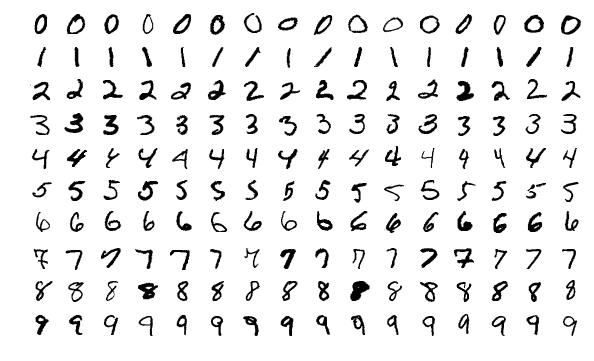
\includegraphics[width=0.75\textwidth]{content/section01/chapter01/figs/mnist.jpg}
    \caption{Sample images from the MNIST dataset.}
    \label{fig:mnist-samples}
\end{figure}

To begin, we import the essential PyTorch modules required for defining neural networks, optimization, dataset loading, and data transformation. The MNIST dataset is automatically downloaded in the original \texttt{.gz} compressed \texttt{ubyte} format. 

We apply a sequence of transformations: first converting each image to a PyTorch tensor, and then normalizing it using the dataset’s mean and standard deviation. The \texttt{DataLoader} wraps the dataset into iterable mini-batches and shuffles the training data at each epoch to improve learning.

\begin{tcolorbox}[codebox]
\begin{verbatim}
import torch
import torch.nn as nn
import torch.optim as optim

from torchvision import datasets, transforms
from torch.utils.data import DataLoader

transform = transforms.Compose([
    transforms.ToTensor(),
    transforms.Normalize((0.1307,), (0.3081,))
])

train_dataset = datasets.MNIST(root='./data', train=True, download=True, \
    transform=transform)

train_loader = DataLoader(train_dataset, batch_size=64, shuffle=True)

test_dataset = datasets.MNIST(root='./data', train=False, download=True, \
    transform=transform)

test_loader = DataLoader(test_dataset, batch_size=1000, shuffle=False)
\end{verbatim}
\end{tcolorbox}

We define a feedforward neural network by creating a subclass of \texttt{nn.Module}, which is the base class for all neural networks in PyTorch. The network structure is specified in two parts. 
\begin{itemize}
    \item The \texttt{\_\_init\_\_} method initializes the layers of the network. Here, the input layer is a fully connected linear layer that maps the \(28 \times 28 = 784\) input pixels to 128 hidden units. This is followed by a second hidden layer with 64 units, and finally an output layer with 10 units, corresponding to the ten digit classes (0 through 9).
    
    \item The \texttt{forward} method defines the forward pass computation. The input image is first flattened to a vector of size 784. Then it is passed sequentially through the linear layers and ReLU activation functions. Specifically, the ReLU activation is applied after the first and second linear transformations to introduce non-linearity, while the final output layer produces raw scores (logits) without an activation function, typically used with \texttt{CrossEntropyLoss}.
\end{itemize}

This architecture allows the model to learn a non-linear mapping from image pixels to digit class scores using two hidden layers.

\begin{tcolorbox}[codebox]
\begin{verbatim}
class FeedforwardNN(nn.Module):
    def __init__(self):
        super(FeedforwardNN, self).__init__()
        self.fc1 = nn.Linear(28*28, 128)
        self.relu = nn.ReLU()
        self.fc2 = nn.Linear(128, 64)
        self.fc3 = nn.Linear(64, 10)

    def forward(self, x):
        x = x.view(-1, 28*28)
        x = self.fc1(x)
        x = self.relu(x)
        x = self.fc2(x)
        x = self.relu(x)
        x = self.fc3(x)
        return x

model = FeedforwardNN()
\end{verbatim}
\end{tcolorbox}

Next, we define the loss function and optimizer. We use \texttt{CrossEntropyLoss}, which internally applies \texttt{LogSoftmax} followed by negative log-likelihood loss. For optimization, we use the Adam algorithm.

\begin{tcolorbox}[codebox]
\begin{verbatim}
criterion = nn.CrossEntropyLoss()
optimizer = optim.Adam(model.parameters(), lr=0.001)
\end{verbatim}
\end{tcolorbox}

We train the model for 5 epochs. In each iteration over the training data, we first set the model to training mode using \texttt{model.train()}. For each mini-batch, we clear the accumulated gradients from the previous step using \texttt{optimizer.zero\_grad()}, perform a forward pass to compute the predictions, and then compute the loss using the specified loss function. 

The backpropagation step is triggered by \texttt{loss.backward()}, which computes the gradients of the loss with respect to the model parameters. These gradients are then used by the optimizer to update the model parameters via \texttt{optimizer.step()}. A log of the loss is printed every 100 batches to monitor training progress.


\begin{tcolorbox}[codebox]
\begin{verbatim}
num_epochs = 5
for epoch in range(num_epochs):
    model.train()
    for batch_idx, (data, target) in enumerate(train_loader):
        optimizer.zero_grad()
        output = model(data)
        loss = criterion(output, target)
        loss.backward()
        optimizer.step()
        if batch_idx % 100 == 0:
            print(f"Epoch [{epoch+1}/{num_epochs}], \
                Batch [{batch_idx}/{len(train_loader)}], Loss: {loss.item():.4f}")
\end{verbatim}
\end{tcolorbox}


After training, we evaluate the model’s accuracy on the test set. We disable gradient computation and compare predicted labels with true labels to count the correct predictions.

\begin{tcolorbox}[codebox]
\begin{verbatim}
model.eval()
correct = 0
total = 0
with torch.no_grad():
    for data, target in test_loader:
        outputs = model(data)
        _, predicted = torch.max(outputs.data, 1)
        total += target.size(0)
        correct += (predicted == target).sum().item()

print(f'Test Accuracy of the model on 10,000 test images: \
    {100 * correct / total:.2f}%')
\end{verbatim}  
\end{tcolorbox}


The trained model achieves an accuracy of approximately \textbf{97.65\%} on the MNIST test dataset. 

This confirms that even a basic feedforward neural network, when trained appropriately using backpropagation, can effectively learn to classify digits from images.